\documentclass[a4paper,12pt]{article}

%%% Работа с русским языком
\usepackage{cmap}					% поиск в PDF
\usepackage{mathtext} 				% русские буквы в формулах
\usepackage[T2A]{fontenc}			% кодировка
\usepackage[utf8]{inputenc}			% кодировка исходного текста
\usepackage[english,russian]{babel}	% локализация и переносы
\usepackage{xcolor}
\usepackage{hyperref}
 % Цвета для гиперссылок
\definecolor{linkcolor}{HTML}{799B03} % цвет ссылок
\definecolor{urlcolor}{HTML}{799B03} % цвет гиперссылок

\hypersetup{pdfstartview=FitH,  linkcolor=linkcolor,urlcolor=urlcolor, colorlinks=true}

%%% Дополнительная работа с математикой
\usepackage{amsfonts,amssymb,amsthm,mathtools} % AMS
\usepackage{amsmath}
\usepackage{icomma} % "Умная" запятая: $0,2$ --- число, $0, 2$ --- перечисление

%% Номера формул
%\mathtoolsset{showonlyrefs=true} % Показывать номера только у тех формул, на которые есть \eqref{} в тексте.

%% Шрифты
\usepackage{euscript}	 % Шрифт Евклид
\usepackage{mathrsfs} % Красивый матшрифт

%% Свои команды
\DeclareMathOperator{\sgn}{\mathop{sgn}}

%% Перенос знаков в формулах (по Львовскому)
\newcommand*{\hm}[1]{#1\nobreak\discretionary{}
{\hbox{$\mathsurround=0pt #1$}}{}}
% графика
\usepackage{graphicx}
\graphicspath{{pictures/}}
\DeclareGraphicsExtensions{.pdf,.png,.jpg}
\author{Бурмашев Григорий, БПМИ-208}
\title{Вычислимость и сложность. Дз -- 1. Вариант -- 1}
\date{\today}
\begin{document}
\maketitle
\clearpage
\section*{Номер 1}
\[
K = \{ a, b\}
\]
Строим элементарную формальную систему, описание предикатов ниже
\[
Q_{(aa, b)}
\]
\[
Q_{(ab, a)}
\]
\[
Q_{(ba, a)}
\]
\[
Q_{(x, y)} \rightarrow Q_{(y, x)}
\]
\[
Q_{(x, y)} \rightarrow Q_{(xb, yaa)}
\]
\[
Q_{(x, y)} \rightarrow Q_{(xb, aay)}
\]
\[
Q_{(x, y)} \rightarrow Q_{(bx, yaa)}
\]
\[
Q_{(x, y)} \rightarrow Q_{(bx, aay)}
\]
\[
Q_{(x, y)} \rightarrow Q_{(xba, ya)}
\]
\[
Q_{(x, y)} \rightarrow Q_{(xba, ay)}
\]
\[
Q_{(x, y)} \rightarrow Q_{(bax, ya)}
\]
\[
Q_{(x, y)} \rightarrow Q_{(xab, ya)}
\]
\[
Q_{(x, y)} \rightarrow Q_{(xba, ya)}
\]
\[
Q_{(x, y)} \rightarrow Q_{(bax, ay)}
\]
\[
Q_{(x, y)} \rightarrow Q_{(abx, ya)}
\]
\[
Q_{(x, y)} \rightarrow Q_{(abx, ay)}
\]
\[
Q_{(x, y)} \rightarrow Q_{(axb, ay)}
\]
\[
Q_{(x, y)} \rightarrow Q_{(axb, ya)}
\]
\[
Q_{(x, y)} \rightarrow Q_{(axa, yb)}
\]
\[
Q_{(x, y)} \rightarrow Q_{(axa, by)}
\]
\[
Q_{(x, y)} \rightarrow Q_{(bxa, ay)}
\]
\[
Q_{(x, y)} \rightarrow Q_{(bxa, ya)}
\]
\[
Q_{(x, y)} \rightarrow P_{xy}
\]
$P$ - одноместный предикатный символ, который представляет само искомое множество $W$ (такие слова, что a в два раза больше, чем b)
\\
$Q$ - двуместный предикатный символ, который отвечает за такие пары $(x, y)$, где слова $x$, $y$ состоят из символов $a, b$, а если просуммировать количество a и b в обоих элементах кортежа, то получится, что символов a в два раза больше, чем символов b
\clearpage
\section*{Номер 2}
Хотим:
\begin{center}

\includegraphics[scale=0.5]{1.png}
\end{center}
Распишем нашу функцию с помощью известных нам базовых перечислимых отношений. Можем заметить, что если $x$ -- четный, то 2 будет являться делителем $x$ (очевидный факт). Тогда можем представить нашу функцию как:
\[
y = (y = (x + 1) \wedge 2 \; | \; x) \vee (y = (x - 1) \wedge 2 \nmid x)
\]
Что расшифровывается как: $y$ равно $x + 1$, если $x$ делится на 2, или $y = x -1$, в случае если $x$ \textbf{не} делится на 2. 
Теперь вспоминаем, 
что на семинаре номер 2, в задаче номер 3, пункт (в) мы доказали разрешимость:
\[
x + y = z
\]
Отсюда получаем разрешимость $y = (x + 1)$ и $y = (x - 1)$. А на семинаре номер 2, в задаче номер 6 мы доказали перечислимость:
\[
x \; | \; y 
\]
Отсюда получаем перечислимость $ 2 \; | \; x$ и $2 \; \nmid x $. На семинаре номер 2, в задаче номер 4 мы доказали перечислимость обьединений и пересечений. Мы смогли расписать через перечислимые отношения, а значит график нашей функции перечислим, а отсюда и сама функция вычислима по Смаллиану
\begin{center}
\textbf{Ч.Т.Д} 
\end{center}
\clearpage
\section*{Номер 3}
\begin{center}
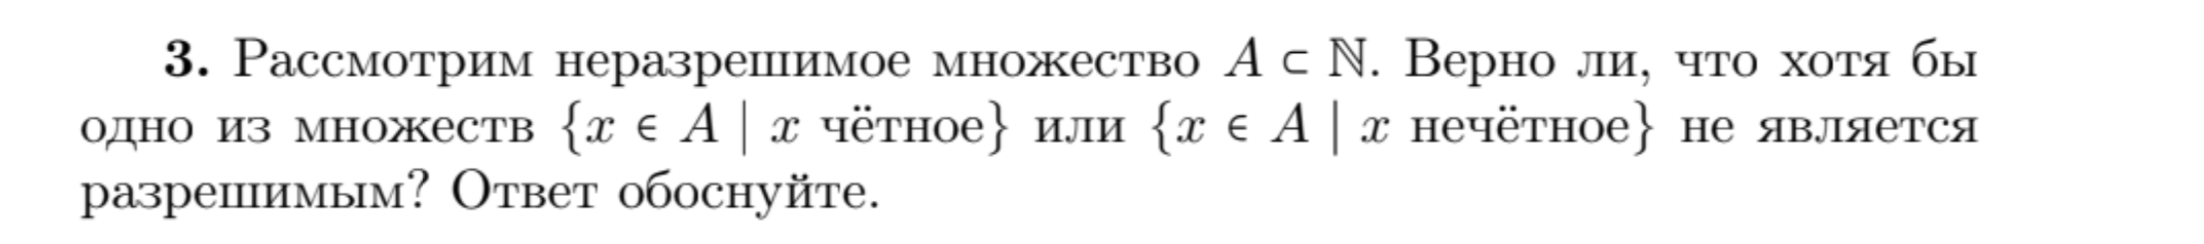
\includegraphics[scale=0.4]{3.png}
\end{center}
Решим от обратного, предположим, что оба множества разрешимы. Тогда посмотрим на их объединение. Во первых вспомним, что объединение двух разрешимых множеств есть разрешимое множество (доказывали на лекции), а во вторых заметим, что объединение этих множеств образует само множество A (потому что мы смотрим все $x$, которые лежат в A, как чётные, так и нечётные, ну а других чисел у нас просто нет). Но тогда мы приходим к противоречию, ведь по условию задачи множество A является неразрешимым, а отсюда из противоречия получаем, что хотя бы одно из двух множеств является неразрешимым, т.е \textbf{не} является разрешимым
\begin{center}
\textbf{Ответ: } да, верно
\end{center}
\end{document}
